\documentclass{beamer}

\usepackage{graphicx} % insert picture
\usepackage{listings}
\usepackage{natbib} % Harvard reference format
\usepackage{hyperref}
\usepackage{tikz} % draw a text structure

\definecolor{github-light-bg}{RGB}{255, 255, 255}
\definecolor{github-light-fg}{RGB}{3, 102, 214}
\definecolor{github-light-yellow}{RGB}{128, 102, 0}
\definecolor{github-light-orange}{RGB}{170, 0, 17}
\definecolor{github-light-purple}{RGB}{102, 51, 153}
\definecolor{github-light-cyan}{RGB}{0, 128, 128}
\definecolor{github-light-green}{RGB}{0, 128, 0}
\definecolor{github-light-red}{RGB}{204, 0, 0}

\lstdefinestyle{githublight}{
	backgroundcolor=\color{github-light-bg},
	basicstyle=\color{github-light-fg}\ttfamily,
	commentstyle=\color{github-light-green},
	keywordstyle=\color{github-light-purple},
	numberstyle=\tiny\color{github-light-fg},
	stringstyle=\color{github-light-cyan},
	identifierstyle=\color{github-light-orange},
	emphstyle=\color{github-light-red},
	emph={[2]TRUE,FALSE},
	emphstyle={[2]\color{github-light-yellow}},
	breaklines=true,
	breakatwhitespace=true,
	numbers=left,
	numbersep=5pt,
	stepnumber=1,
	showstringspaces=false,
	frame=single,
	rulecolor=\color{github-light-fg},
	framerule=0.5pt,
	tabsize=4,
	columns=flexible,
	extendedchars=true,
	inputencoding=utf8,
	upquote=true,
}

\lstset{style=githublight}

\usetheme{metropolis}
\title{Trading Liberties: \\
Estimating COVID-19 Policy Preferences from Conjoint Data}
\date{\today}
\author{Author: Felix Hartmann et al \\
Replication Author: Chenxi Li}
\institute{Trinity College Dublin\\College Green, Dublin 2 \\ \par Lic8@tcd.ie}
\begin{document}
\maketitle
\section{Research Background}

\begin{frame}{Research Question}
	\noindent The research questions of this paper are:
	\begin{itemize}
		\item[-] In which conditions citizens support restricting freedoms?
		\item[-] How such restrictions affect trust in political institutions?
	\end{itemize}
\end{frame}

\begin{frame}{Research Review}
\noindent What we already known are:
\begin{itemize}
	\item[-] citizens are willing to trade individual liberties for security in light of an external threat \citep{davis2004civil}
	\item[-] Regarding COVID-19, citizens with higher health related insecurity are more willing to sacrifice civil liberties \citep{stantcheva2020civil}
\end{itemize}
\end{frame}

\begin{frame}{Research Conclusions}
\noindent And what we can conclude are:
\begin{itemize}
	\item[-] There is a greater acceptance of more strict policies when severity increases.
	\item[-] Vaccinated citizens will strongly support stringent policies in extreme conditions.
	\item[-] Also, Vaccinated citizens will differentiate between vaccinated and unvaccinated fellow citizens and are most likely to support restrictions for unvaccinated people only.  
\end{itemize}
\end{frame}

\section{Variables Introduction}

\begin{frame}{Dependent Variable}
	\noindent In this paper, we have 4 different regression models, which refers to 4 different dependent variables $Y$.
	\par
	\begin{itemize}
		\item[-] $Y_{choice}$: A binary variable measuring which policy the interviewers prefer. And in this case, the author points out 2 policies to choose (0/1).
		\item[-] $Y_{rating}$: The rating to these two proposals (0-10).
		\item[-] $Y_{trust}$: Their trust to the federal government (0-10).
		\item[-] $Y_{probability}$: The probability of acccepting vaccinated for non-vaccinated interviewers. 
	\end{itemize}
\end{frame}

\begin{frame}{Independent Variables}
\begin{itemize}
	\item[1.] Pandemic Severity
	\begin{enumerate}
		\item[-] Moderate worsening (7-day-incidence 150, intensive care bed occupancy 80\%)
		\item[-] Sharp worsening (... 300, ... 90\%)
		\item[-] Dramatic worsening (... 800, ... 100\%)
	\end{enumerate}
	\item[2.] Policy Stringency
	\begin{enumerate}
		\item[-]  Least restrictions (masks)
		\item[-]  Moderate restrictions (plus limitations on social events)
		\item[-]  Most restrictions (plus broader limitations on movements)
	\end{enumerate}
	\item[3.] Policy Universality
	\begin{enumerate}
		\item[-] Most exemptions (restrictions do not apply to vaccinated, recovered, or tested citizens)
		\item[-] Some exemptions (... vaccinated or recovered citizens)
		\item[-] Fewest exemptions (... all citizens)
	\end{enumerate}
\end{itemize}
\end{frame}

\begin{frame}{Regression Formula}
	So we can get our regression formula:
	\begin{align*}
		Y_{it} &= \beta_0 + \beta_1 Z_1 + \beta_2 Z_2 + \beta_3 Z_3 \\
		&\quad + \textcolor{red}{\textbf{$\beta_3$}} Z_1 Z_2 + \beta_4 Z_1 Z_3 + \beta_5 Z_2 Z_3 \\
		&\quad + \beta_6 Z_1 Z_2 Z_3 + u_i + \varepsilon_{it}
	\end{align*}
	\noindent Here, the author made a mistake which wrote $\beta_3$ twice.
	\par
	\noindent Where $Z_1$ represents severity, $Z_2$ represents stringency, and $Z_3$ represents universality \citep{hartmann2024trading}.
\end{frame}

\section{Research Approach}

\begin{frame}{Code - Prepare the Variables}
	\noindent Let's see the code in \texttt{R}. These code is used to prepare for the independent variable including interactions.
	\lstinputlisting[language=R, basicstyle=\footnotesize, firstline=1, lastline=12]{replication.R}
\end{frame}

\begin{frame}{Code - Fit the Model}
\noindent Let's see the code in \texttt{R}. These code is used to fit the regression model, and we can see details through this block:
\lstinputlisting[language=R, basicstyle=\footnotesize, firstline=15, lastline=22]{replication.R}
\end{frame}

\begin{frame}{Code - Fit the Model}
\noindent Also, the author calculate the probability of acccepting vaccinated.
\lstinputlisting[language=R, basicstyle=\footnotesize, firstline=41, lastline=43]{replication.R}
\end{frame}

\begin{frame}{Code - Check the Model}
\noindent Now, let's check one of the model. For example, if we want to check when $Y$ is rating in unvaccinated group, then we can write:
\lstinputlisting[language=R, basicstyle=\footnotesize, firstline=23, lastline=23]{replication.R}
\noindent And then we will see the outputs from \texttt{R}:
\end{frame}
\begin{frame}{Code - Check the Model}
\begin{table}[h]
    \centering
    \caption{Coefficient and Significant of $Y$ = Rating Regression}
    \begin{tabular}{lccc}
        \hline
        & Estimate & Std. Error & Pr($>|t|$)\\
        \hline
        severity & 0.002545 & 0.005734 & 6.572e-01\\
        universality & -0.021862 & 0.005951 & 2.417e-04\\
        stringency & -0.091130 & 0.005649 & 4.293e-57\\
        severity:universality & -0.004736 & 0.007526 & 5.292e-01\\
        severity:stringency & 0.026078 & 0.006853  & 1.435e-04\\
        universality:stringency & 0.001157 & 0.007251 & 8.733e-01\\
        severity:universality:stringency & 0.004653 & 0.008978 & 6.043e-01\\
        \hline
    \end{tabular}
\end{table}
\end{frame}

\begin{frame}{Regression Model}
\noindent So in the upon case, we can write our regression formula:
\begin{align*}
	Y_{rating} &= 0.00 Z_1 - 0.02 Z_2 - 0.09 Z_3 \\
	&\quad + 0.00 Z_1 Z_2 + 0.02 Z_1 Z_3 + 0.00 Z_2 Z_3 \\
	&\quad + 0.00 Z_1 Z_2 Z_3
\end{align*}
\noindent Where $Z_1$ represents severity, $Z_2$ represents stringency, and $Z_3$ represents universality.
\end{frame}

\section{Results Visualisation}
\begin{frame}{Coefficient Visualisation}
\lstinputlisting[language=R, basicstyle=\footnotesize, firstline=25, lastline=39]{replication.R}
\end{frame}

\begin{frame}{Coefficient Visualisation}
\noindent Follow the author's code, we can make this visualisation:
\par
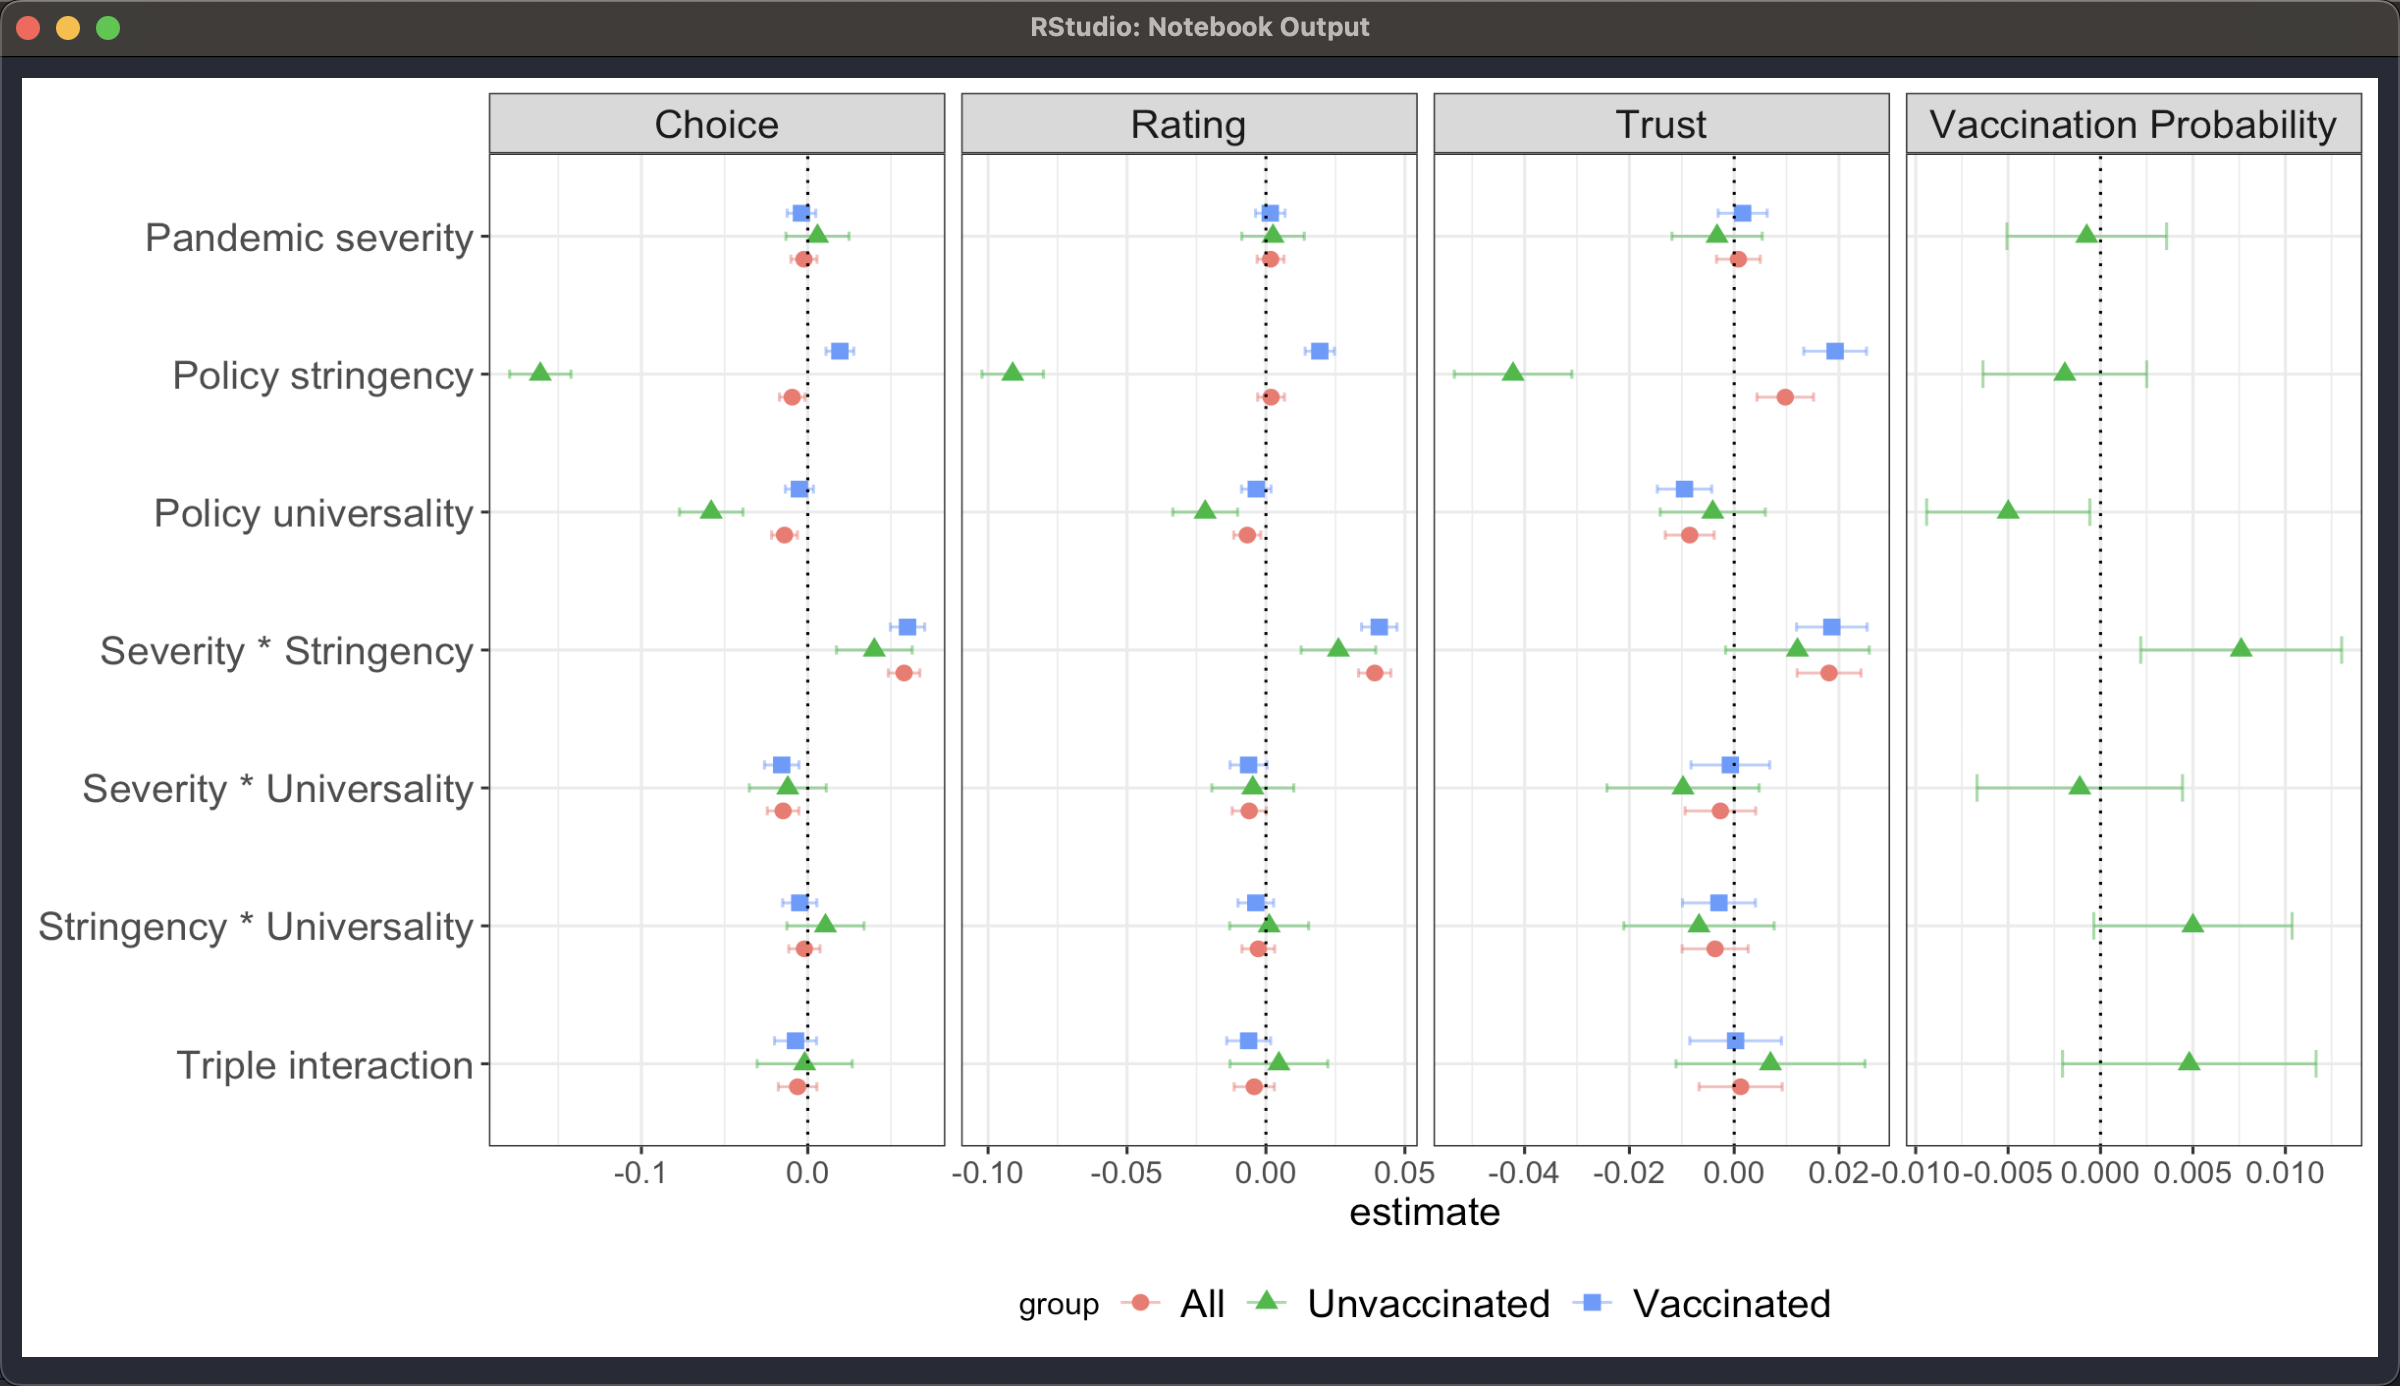
\includegraphics[width=1.05\textwidth]{reg_results.png}
\end{frame}

\begin{frame}{Key Conclusions}
\begin{itemize}
	\item[-] Severity*Stringency: Citizens strongly prefer more severe policies when conditions are bad. Also we can say, there is a clear evidence that citizens are more supportive of more stringent policies as conditions worsen.
	\item[-] Greater stringency is associated with greater willingness to vaccinate.
	\item[-] Severity*Universality: Citizens are still less supportive of universal restrictions (with fewest exemptions) when conditions are bad.
	\item[-] There is no evidence for interactions between the stringency and universality of conditions or for three-way interactions. 
\end{itemize}

\end{frame}

\bibliographystyle{agsm}

\begin{frame}{Literature List}
\bibliography{mybibliography}

\end{frame}

\end{document}